\documentclass{article}

% Language setting
\usepackage[italian]{babel}
\usepackage[utf8]{inputenc}
\usepackage[T1]{fontenc}

% Set page size and margins
\usepackage[letterpaper,top=1.9cm,bottom=1.9cm,left=3cm,right=3cm,marginparwidth=1.75cm]{geometry}

% Useful packages
\usepackage{amsmath}
\usepackage{graphicx}
\usepackage{booktabs}
\usepackage{siunitx}
\usepackage[colorlinks=true, allcolors=blue]{hyperref}

\graphicspath{{figures/}}

\linespread{0.94}

% Tighten float/caption spacing and let floats pack densely, to keep the
% report within two pages.
\setlength{\textfloatsep}{7pt plus 2pt minus 2pt}
\setlength{\intextsep}{7pt plus 2pt minus 2pt}
\setlength{\abovecaptionskip}{4pt}
\setlength{\belowcaptionskip}{2pt}
\renewcommand{\topfraction}{0.92}
\renewcommand{\bottomfraction}{0.9}
\renewcommand{\textfraction}{0.05}
\renewcommand{\floatpagefraction}{0.7}
\setcounter{topnumber}{3}
\setcounter{bottomnumber}{2}
\setcounter{totalnumber}{5}

\title{RSNA Pediatric Bone Age Challenge (2017)}
\author{Vittoriana Sanna}
\date{}

\begin{document}
\maketitle
\vspace{-2em} 

\section{Introduzione}

La maturità scheletrica è un parametro importante nella radiologia pediatrica. Per valutarla, di solito si confronta una radiografia della mano sinistra con delle immagini di riferimento. Tuttavia, questo metodo può essere lento e soggettivo, poiché diversi osservatori possono avere opinioni diverse.
Per superare questo limite, la RSNA \cite{rsna2017} Pediatric Bone Age Challenge del 2017 ha proposto di affrontare il problema mediante un modello di apprendimento supervisionato. In particolare, l'obiettivo è quello di stimare, attraverso una tecnica di regressione, l'età ossea del paziente espressa in mesi, partendo da una radiografia della mano e dal sesso del paziente. Il sesso è importante perché i maschi e le femmine hanno tempi di sviluppo scheletrico diversi. Quindi, la stessa radiografia può corrispondere a età diverse a seconda del sesso.
Per risolvere questo problema, è stata utilizzata una rete neurale convoluzionale bidimensionale personalizzata. Questa rete è in grado di estrarre caratteristiche visive dalla radiografia e di combinarle con l'informazione sul sesso del paziente. La combinazione avviene attraverso una tecnica chiamata fusione tardiva (\emph{late fusion}). Dopo aver preparato i dati, la rete è stata addestrata con un protocollo di hold-out, che prevede la suddivisione del dataset in tre insiemi distinti: training, validation e test. Il training set è utilizzato per l'apprendimento del modello, il validation set per monitorarne le prestazioni e selezionare la configurazione migliore, mentre il test set viene impiegato esclusivamente per la valutazione finale su dati mai utilizzati durante l'addestramento. Il modello finale è stato scelto tra quattro opzioni diverse, in base al suo errore di validazione.

\section{Preprocessing}

A partire dalle radiografie grezze in scala di grigi, ogni immagine segue una serie di passaggi prima di arrivare alla rete (Figura~\ref{fig:prep}). Il primo passo è quello di riempire l'immagine con zeri fino a renderla quadrata, sfruttando il fatto che lo sfondo della radiografia è scuro. Ciò serve a evitare che il successivo ridimensionamento a $256\times256$ pixel distorca le proporzioni della mano.
Dopo questo passo, si applica la tecnica di Contrast Limited Adaptive Histogram Equalization, nota come CLAHE. Questa tecnica migliora il contrasto dell'immagine in modo locale, accentuando i bordi delle ossa e le cartilagini di accrescimento. Questi ultimi sono particolarmente importanti perché contengono gran parte del segnale che indica l'età.

\begin{figure}[htbp]
\centering
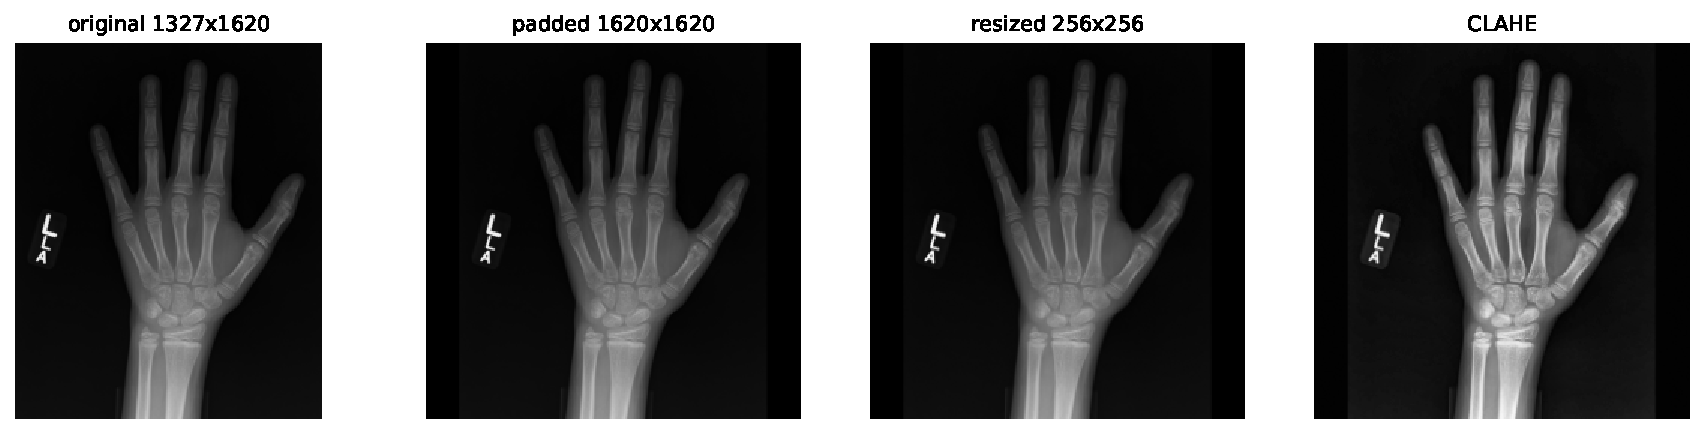
\includegraphics[width=0.82\linewidth]{preprocessing.pdf}
\caption{Pipeline di preprocessing: padding a quadrato, ridimensionamento a $256\times256$, CLAHE.}
\label{fig:prep}
\end{figure}

Si applicano due operazioni di normalizzazione per rendere il processo di addestramento più stabile. La prima riguarda i valori di intensità dei pixel delle immagini, che vengono normalizzati utilizzando la media $0.184$ e la deviazione standard $0.212$, calcolate sul training set. La seconda riguarda il target (l'età ossea), ossia il valore che il modello deve imparare a prevedere. Anche in questo caso vengono utilizzate le statistiche del training set ($127.3\pm41.2$ mesi), così che il modello lavori con valori su una scala più adatta all'apprendimento. Al termine dell'addestramento, le predizioni del modello vengono riconvertite nella scala originale, così da ottenere direttamente l'età ossea espressa in mesi.
Per migliorare la capacità del modello di analizzare nuove immagini, solo le immagini del training set vengono sottoposte a data augmentation, cioè a leggere trasformazioni casuali che simulano le normali variazioni presenti nelle radiografie. In particolare, vengono applicate rotazioni casuali fino a $\pm20^\circ$, piccole variazioni di scala (con fattore compreso tra $0.9$ e $1.1$), traslazioni e lievi modifiche della luminosità e del contrasto fino a $\pm0.2$. Queste trasformazioni aumentano la variabilità dei dati di addestramento senza alterare in modo significativo le proporzioni scheletriche della mano, rendendo il modello più robusto nell'analizzare nuove immagini.

\section{Modello}

La rete neurale utilizzata, denominata \texttt{BoneAgeCNN}, è composta da circa $4.49$ milioni di parametri, ossia i valori che il modello modifica durante l'addestramento per imparare a stimare l'età ossea.
L'architettura della rete si ispira al modello proposto da Cole et al.~\cite{cole2017} ed è costituita da un estrattore di caratteristiche formato da cinque blocchi consecutivi, ciascuno composto da una $\text{Convoluzione }{3\times3}$, seguita da una funzione di attivazione ReLU, una seconda $\text{Convoluzione }{3\times3}$, un livello di Batch Normalization, un'ulteriore funzione ReLU e, infine, un'operazione di Max Pooling $2\times2$. 
Man mano che l'immagine attraversa i cinque blocchi, la rete costruisce progressivamente rappresentazioni sempre più complesse della radiografia. Parallelamente, le operazioni di Max Pooling riducono progressivamente la dimensione delle rappresentazioni interne, conservando le informazioni più importanti e diminuendo il numero di calcoli necessari per la rete.
Al termine di questo processo, tutte le caratteristiche estratte vengono riassunte in un unico vettore numerico che rappresenta una sintesi della radiografia. A questo vettore viene aggiunta l'informazione relativa al sesso del paziente mediante una strategia di fusione tardiva.
Le caratteristiche estratte dalla radiografia, insieme all'informazione relativa al sesso del paziente, vengono quindi passate alla parte finale della rete, chiamata regressore. Questa parte combina le informazioni disponibili e produce un unico valore numerico, corrispondente all'età ossea stimata. Durante questa fase viene utilizzato il dropout, una tecnica che disattiva casualmente una parte dei neuroni durante l'addestramento per ridurre il rischio di overfitting e migliorare la capacità del modello di analizzare nuove immagini.

Nel corso dell'addestramento, ogni previsione viene confrontata con l'età ossea reale attraverso una funzione di perdita L1, che calcola l'errore assoluto tra il valore predetto e quello corretto. L'obiettivo della rete è ridurre progressivamente questo errore aggiornando i propri parametri a ogni iterazione.

\section{Impostazione sperimentale}

Il dataset totale viene suddiviso una sola volta in tre gruppi separati, seguendo un protocollo hold-out: $12{.}611$ immagini per il training, $800$ immagini per la validazione e $625$ immagini per il test. Per confrontare le diverse configurazioni della rete, sono state mantenute costanti alcune condizioni sperimentali: la risoluzione delle immagini in ingresso ($256\times256$), la dimensione del batch ($32$), il numero di epoche ($30$), il weight decay ($5\times10^{-5}$) e il decadimento esponenziale del learning rate ($\gamma=0.97$). Durante l'addestramento, il modello aggiorna progressivamente i propri parametri cercando di ridurre l'errore di previsione.

Sono state confrontate quattro configurazioni della rete, modificando alcuni aspetti dell'architettura e del processo di addestramento per individuare la soluzione più efficace. La configurazione \texttt{baseline} rappresenta il modello di riferimento, con cinque blocchi, dropout pari a $0.3$ e ottimizzatore SGD~\cite{goodfellow2016}. La configurazione \texttt{high\_dropout} mantiene la stessa architettura ma aumenta il dropout a $0.5$, con l'obiettivo di ridurre il rischio di overfitting. La configurazione \texttt{shallow} utilizza invece una rete più semplice, composta da quattro blocchi, per valutare se una struttura meno complessa possa ottenere risultati comparabili. Infine, la configurazione \texttt{adam} utilizza l'ottimizzatore Adam~\cite{kingma2015adam} al posto di SGD, modificando il metodo con cui vengono aggiornati i parametri della rete durante l'apprendimento. 
La configurazione finale viene selezionata sulla base dell'errore ottenuto sul validation set, scegliendo il modello con le migliori capacità di funzionare su immagini mai viste.

Le prestazioni dei modelli sono state valutate utilizzando due metriche, entrambe espresse in mesi. La prima è l'errore assoluto medio (MAE, Mean Absolute Error), che rappresenta l'errore medio tra l'età ossea predetta e quella reale ed è la metrica principale utilizzata durante l'addestramento. La seconda è la radice dell'errore quadratico medio (RMSE, Root Mean Square Error), una metrica più sensibile agli errori grandi rispetto al MAE. Per questo motivo è utile per verificare se il modello presenta alcune predizioni con errori particolarmente elevati.

\section{Risultati}
La Tabella~\ref{tab:ablation} mostra i risultati finali dell'addestramento e della validazione delle quattro diverse configurazioni. La configurazione \texttt{adam} ha ottenuto i risultati migliori ed è stata scelta come modello finale, mentre \texttt{shallow} e \texttt{high\_dropout} hanno mostrato prestazioni inferiori, indicando una minore capacità di apprendimento entro le 30 epoche disponibili.

\begin{table}[htbp]
\centering
\begin{tabular}{lrr}
\toprule
Configurazione & Perdita train & Perdita valid \\
\midrule
\texttt{adam}         & 0.231 & 0.240 \\
\texttt{baseline}     & 0.280 & 0.283 \\
\texttt{high\_dropout} & 0.568 & 0.468 \\
\texttt{shallow}      & 0.679 & 0.669 \\
\bottomrule
\end{tabular}
\caption{Ablazione sulle quattro configurazioni (perdita L1, target standardizzato).}
\label{tab:ablation}
\end{table}

Il modello selezionato raggiunge un errore assoluto medio (MAE) sul test set pari a circa $8.15$ mesi, come mostrato nella Tabella~\ref{tab:metrics}. Gli errori di training, validazione e test sono tra loro simili, indicando che il modello riesce a generalizzare bene anche su immagini non utilizzate durante l'addestramento.

\begin{table}[htbp]
\centering
\begin{tabular}{lrr}
\toprule
Split & MAE (mesi) & RMSE (mesi) \\
\midrule
Train & 8.68 & 11.51 \\
Valid & 9.89 & 13.77 \\
Test  & 8.15 & 10.70 \\
\bottomrule
\end{tabular}
\caption{Errore del modello migliore (\texttt{adam}) su ciascuno split.}
\label{tab:metrics}
\end{table}

Durante l'addestramento, è stato inoltre analizzato l'andamento della funzione di perdita sui dati di training e di validazione. La curva relativa al training set mostra come l'errore diminuisca progressivamente mentre il modello apprende dalle immagini utilizzate per l'addestramento, mentre la curva di validazione permette di verificare se questo miglioramento viene mantenuto anche su immagini non utilizzate durante il training.
La storia della perdita (Figura~\ref{fig:loss}) mostra una progressiva riduzione dell'errore durante l'addestramento. Il valore minimo della validation loss viene raggiunto verso la fine delle 30 epoche, indicando che il modello continua a migliorare per gran parte del processo di training.

Se analizziamo l'errore di test suddiviso per gruppo di età (Figura~\ref{fig:mae}), si osserva che l'errore tende ad aumentare agli estremi dell'intervallo di età considerato, cioè nei soggetti più giovani e in quelli più anziani. Questo comportamento è legato al fenomeno della regressione verso la media, per cui il modello tende a prevedere valori più vicini all'età media presente nel dataset. Di conseguenza, le età estreme risultano più difficili da stimare, soprattutto a causa della minore quantità di immagini disponibili per questi gruppi. La presenza ridotta di soggetti molto giovani o molto anziani porta infatti a una maggiore incertezza nelle previsioni e quindi a un aumento dell'errore di test.

\begin{figure}[htbp]
\centering
\begin{minipage}{0.49\linewidth}
\centering
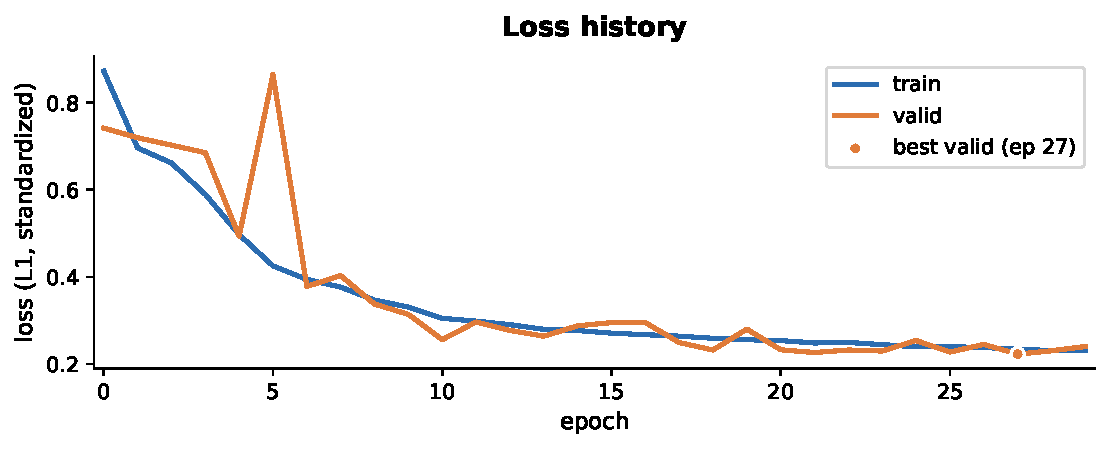
\includegraphics[width=\linewidth]{loss_history.pdf}
\caption{Perdita di training e validazione del modello selezionato.}
\label{fig:loss}
\end{minipage}\hfill
\begin{minipage}{0.49\linewidth}
\centering
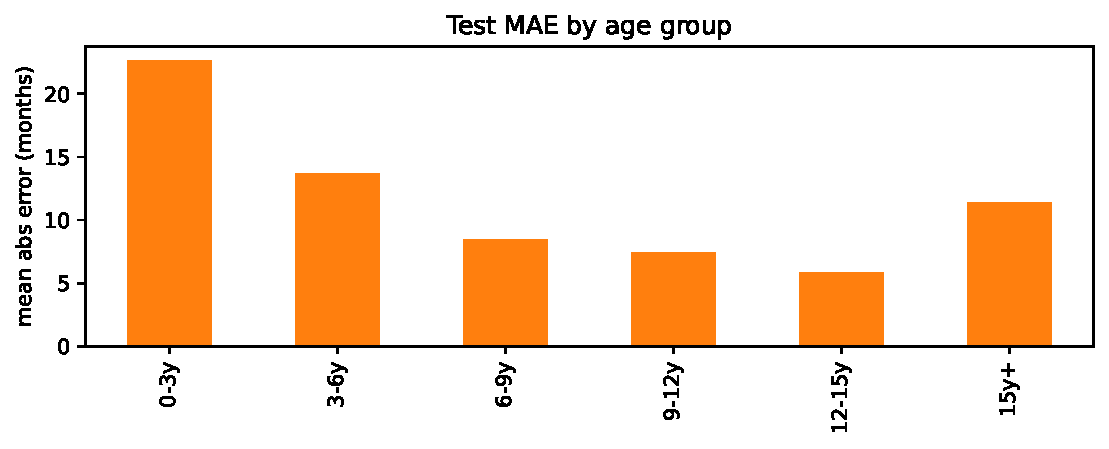
\includegraphics[width=\linewidth]{mae_by_age.pdf}
\caption{MAE di test per gruppo di età.}
\label{fig:mae}
\end{minipage}
\end{figure}

\begin{thebibliography}{9}
\bibitem{cole2017}
J.~H. Cole et al.,
\emph{Predicting brain age with deep learning from raw imaging data}, NeuroImage, 2017.
\bibitem{rsna2017}
Radiological Society of North America,
\emph{RSNA Pediatric Bone Age Challenge}, 2017.
\bibitem{goodfellow2016}
I. Goodfellow, Y. Bengio, and A. Courville,
\emph{Deep Learning},
MIT Press, 2016.
\bibitem{kingma2015adam}
D.~P. Kingma and J. Ba,
\emph{Adam: A Method for Stochastic Optimization},
Proceedings of the International Conference on Learning Representations (ICLR), 2015.
\end{thebibliography}

\end{document}
